\begin{BPMN}{PROC-02}{Creación de una Unidad de Aprendizaje}{}
    \PCitem{Participantes}{}
    \PCitem{Objetivo}{}
    \PCitem{Interrelación con otros procesos}{}
    \PCitem{Proveedores}{}
    \PCitem{Entradas}{}
    \PCitem{Consumidores}{}
    \PCitem{Salidas}{}
    \PCitem{Precondiciones}{}
    \PCitem{Postcondiciones}{}
    \PCitem{Frecuencia}{}
    \PCitem{Tipo}{}
    \PCitem{Áreas de oportunidad}{}
\end{BPMN}
En la figura \hyperref[fig:BPMN-02]{BPMN-02 Proceso para la creación de una Unidad de Aprendizaje}

\begin{figure}[htbp]
	\begin{center}
		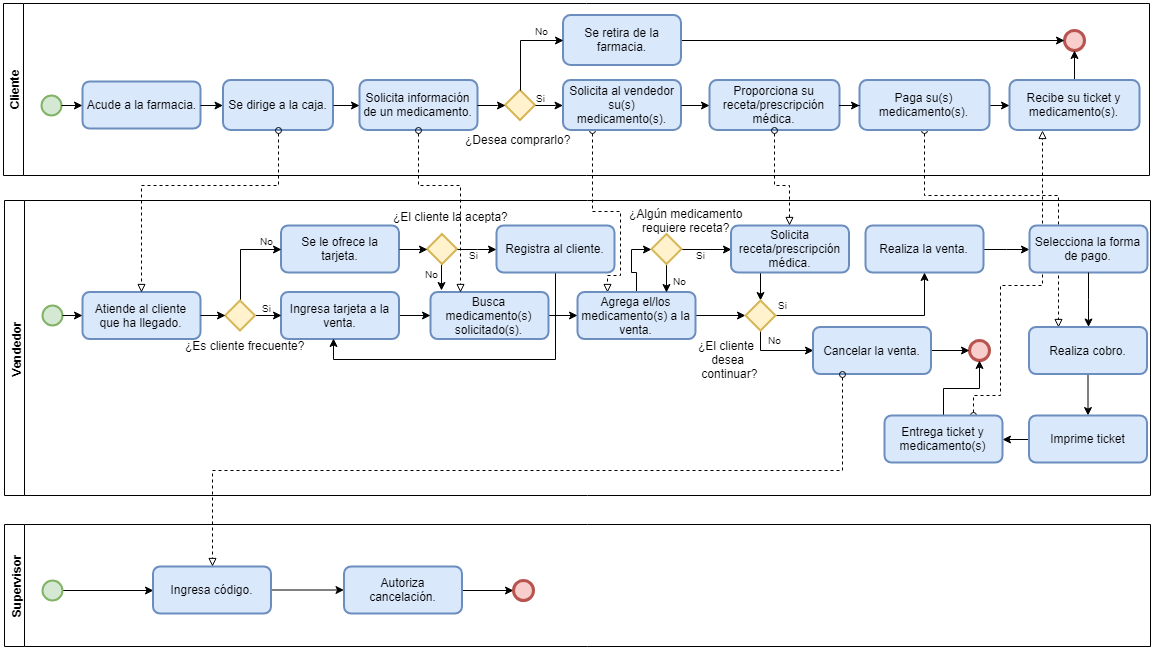
\includegraphics[width=.80\textwidth]{C1-DP/SP1/IG-SP1/BPMN-02}
		\caption{BPMN-02 Proceso para la creación de una Unidad de Aprendizaje}
		\label{fig:BPMN-02}
	\end{center}
\end{figure}
